\section{Implementation Details}
\label{sec:graphene:impl}

\paragraph{Linux \pal{}.}
The majority of \pal{} calls are simple wrappers for similar Linux system calls, 
adding less than 100 LoC on average for translation between \pal{} and Linux abstractions.
The largest \pal{} calls are for exception handling, synchronization, and picoprocess
creation, which require multiple system calls and range from 500--800 LoC each.
Creating a new picoprocesses internally requires a {\tt vfork} and {\tt exec} of a clean 
application instance, and would be more efficiently implemented in the kernel.
Finally, the other major \pal{} components are an ELF loader (2 kLoC), headers (800 LoC),
and internal support code (2.3 kLoC).

\paragraph{Alternative \pal{} Ports.}
We prove the platform independence of \sysname{}
by porting \pal{} to {\em FreeBSD}, {\em OSX} and {\em Windows}.
With the alternative host \pal{}, unmodified Linux binaries,
along with {\tt glibc} and {libLinux},
can be transparently run on the host.
For FreeBSD,
only 1.2 kLoC of the host \pal{} code need to be rewritten,
which are significantly less than FreeBSD Linux compatibility module (10.8 kLoC).
\pal{} components including ELF loader and internal support code can be shared by any \pal{} ports.

%\fix{We leave host \pal{} ports to non-unix OSes like Windows as future work,
%but previous works~\citep{porter11drawbridge,baumann13bascule} have already shown it feasible.}

\begin{table}[t!b!]
\footnotesize
\centering
\begin{tabular}{|l|rr|}
\hline
{\bf Component} & {\bf Lines} & ({\bf \% Changed})\\
\hline
GNU Library C ({\tt libc}, {\tt ld}, {\tt libdl}, {\tt libpthread}) & \libclines{} & $0.07\%$ \\
\hline
Linux Library OS ({\tt libLinux}) & 31,112 & \\
Linux host \pal{} & 11,644 & \\
% updated by Chia-Che on Oct. 10, 2013
\hline
%Storage Server & \fixmedp{XX} & \\
Reference monitor bootstrapper & \reflines{} & \\
Linux kernel reference monitor module ({\tt /dev/graphene}) & \sandboxmodlines{} & \\
Linux kernel IPC module ({\tt /dev/gipc}) & \gipclines{} & \\
\hline
\end{tabular}
\caption[\sysname{}: lines of code written or changed]
{Lines of code written or changed to produce \sysname{}.  Applications and other libraries are unchanged.}
\label{tab:graphene:loc}
\end{table}


%% * most calls are a wrapper, \fixmedp{XX} LoC on average.
%% * Exception handling, sync, and process creation were harder (500-800 LoC each).  Process creation requires a clean instance (vfork+exec), would be simpler to implement in kernel.
%% * Other major components: ELF loader (2kLoC), headers(800 LoC), internal support code (2300 LoC)


%\fixmedp{Chia-Che, update LoC table}

\paragraph{Implementing Linux Personality.} 
%\fixmedp{Revisit the logical flow of these paragraphs}
The \sysname{} {\tt libLinux.so} implements a subset 
of the Linux system call API (currently \syscalls{} calls)
using only the \pal{} ABI to interact with the host.
We note that Linux exports a very long tail of infrequently used calls.
%applications.
A rough analysis of this tail indicates roughly 100 additional calls that can be implemented
with the existing \pal{} ABI and coordination framework, less than 10 administrative calls that will not make sense to expose to 
an application, such as loading a kernel module or rebooting the system, and roughly 54 that will require 
\pal{} extensions to meaningfully implement, such as controlling scheduling,
NUMA placement, I/O privilege, and shared memory.
In the last category of system calls, the degree to which actual host details should be exported versus emulated is debatable.

%We believe represent the most commonly used system calls.
%When an application requests a call or argument that {\tt libLinux.so} does not implement,
%the picoprocess exits with a distinct error message. 
Each time we have tested \sysname{} with a new application, the number of extra system calls
required has dropped---most recently we only added 4 calls
(namely, epoll\_create, epoll\_wait, semget and semop)
to support the Apache web server.
Thus, we believe \sysname{} implements a representative sample of Linux calls.

%such as {\tt sched\_setparam}, which manipulates scheduler-specific
%parameters or 
%{\tt uselib}, which has been abandoned 
%in {\tt glibc} version 2 in favor of a user-space dynamic linker.
%We do not plan to implement administrative interfaces, such as {\tt reboot}.
%The growth in the set of supported system calls has been driven by 
%the requirements of new applications we use to exercise \sysname{}, and has been 
%slowing considerably over time.

%directly to guests, and thus will not implement them in {\tt libLinux.so}.

% dp: :(
\begin{comment}
Most {\tt libLinux.so} code reimplements
Linux kernel functionality.  We found it expedient to 
read the Linux source in order to understand its behavior and then reimplement 
that behavior on the \pal{} ABI in most cases.
In some cases, such as the file caching code,
%directory entry (dentry) cache, 
we refactored code directly from the Linux kernel.
%% In these cases, we simplified data structures to only include data
%% we needed for a single application, and to hook in with other 
%% {\tt libLinux} subsystems.
%% An interesting direction for future work would identify techniques
%% to automatically import larger swaths of Linux kernel code, facilitating
%% adoption of new features and bugfixes.
\end{comment}

In order to use {\tt libLinux.so}, we modified \libclines{} lines of {\tt glibc} to replace 
system instructions with function calls into {\tt lib\-Linux.so},
and to cooperatively manage thread-local storage with {\tt libLinux.so} (Table~\ref{tab:graphene:loc}).

%All totaled, we only needed to modify \libclines{} lines of glibc source code to redirect all 
%system calls to {\tt libLinux} 

%\section{User-level {\tt fork} and other Linux library OS challenges}
%%% \vspace{5pt}
%%% \label{sec:fork}
%%% \noindent {\bf Copy-On-Write Fork.~}
%%% Creating a clean guest eases reasoning about security isolation, as all shared abstractions
%%% must be implemented using explicit data streams  between guests.
%%% This section describes how we implement these Unix abstractions in the guest
%%% %achieve a sensible division of labor between guest and host, and 
%%% without baking Unix personality into the host ABI.


\begin{comment}
\vspace{5pt}
\noindent{\bf Guest self-migration.~}  One of the key features of the host ABI
is that guest state can be programmatically read and recreated.
As a result, guests can checkpoint, migrate, and resume themselves in a new picoprocess,
potentially on a new host.  
Most of the library OS and application state are checkpointed simply 
by copying the contents of virtual memory into a file.
Checkpointing requires manually serializing a few key data structures
in {\tt libLinux} that are needed to resume the library OS from a checkpoint,
% interface directly with the PAL, 
including the thread states, handle table, and memory mappings.  

Resuming from a checkpoint involves restoring these key data
structures (handles, thread register contexts, memory mappings), and re-loading memory
contents from the checkpoint.  Most additional data structures
in {\tt libLinux}, and all application data structures,
are reloaded at the virtual address as before the checkpoint and work without modification.
\end{comment}

\begin{comment}
When a new guest begins execution, an input argument to {\tt libLinux} indicates
whether control should be transferred to the Linux loader ({\tt ld.so}) to start a new application instance, 
or whether a checkpoint should be loaded instead.
\end{comment}
%After the checkpoint is loaded, all threads resume execution on their stacks.

\paragraph{Implementing fork by (Ab)using Checkpoints.} 
Copy-on-write fork presented a particular challenge.
%when implemented using only a VM-like picoprocess abstraction.
As with a virtual machine, each new picoprocess 
is created in a ``clean'' state; fork is implemented in the \libos{}.
%yet applications require common Unix abstractions such as file handle inheritance and copy-on-write fork.

Graphene implements file Unix-style {\tt fork}
by leveraging portions of the checkpoint and migration code,
which can programmatically save and restore OS state (e.g., file handles, and memory mappings).
Rather than writing the checkpoint to a file, 
we developed an efficient bulk IPC mechanism to 
permit copy-on-write sharing of memory pages among processes.
Bulk IPC is a performance optimization over sending each byte of the parent address
space over a stream, although {\tt libLinux} can also implement {\tt fork}
over a stream.
Bulk IPC adds 3 calls to the host ABI,
and the host reference monitor only permits bulk IPC among
picoprocesses within a sandbox.

%% Conceptually, {\tt fork} could be implemented by checkpointing the parent,
%% modifying the primary thread's checkpoint 
%% so that the child returns 0 from the fork call 
%% (indicating it is the child),
%% and then immediately resuming the checkpoint in another picoprocess.

%% In practice, we optimize {\tt fork} performance by avoiding 
%% the use of an intermediate checkpoint file, instead transferring the checkpoint
%% directly to the child over a host-level bulk IPC
%%  mechanism (\S\ref{sec:linux:pal}).
%The Graphene bulk IPC abstraction adds 3 PAL calls 
%that allow guests to efficiently transfer large regions of memory to each other\fixmedp{after reordering, add a forward or back ref}.

Using our bulk IPC mechanism,
the sender (parent) can request that the host kernel copy
a series of pages, which need not be virtually contiguous,
into the receiver's address space.
The receiver (child) specifies where these pages should be mapped.
In both sender and receiver, the pages are marked copy-on-write.  
This bulk IPC mechanism sends pages out-of-band on a byte stream and guests also use the stream to send control messages 
indicating 
how many pages are being sent and how they should be interpreted.

Our IPC module is \gipclines{} lines of code (Table~\ref{tab:graphene:loc}), 
runs on multiple versions of Linux (2.6 and 3 series kernels), and
does not require
Linux kernel changes or recompilation.


\begin{comment}
A critical challenge in developing a Linux library OS was implementing 
handle inheritance in the guest.  In some cases, 
handles are easy to reproduce: an open file can simply be reopened in the child,
and the cursor offset adjusted (note that file handle offsets are a library abstraction
implemented over a memory mapped file).
Pipes, however, are not easily recreated without host support.
\end{comment}
%One option was to create explicitly named host-level byte streams,
%similar to System V or Windows named pipes.
%This strategy is simple to add to the Drawbridge host ABI and easy to program in {\tt libLinux},
%but complicates security isolation, as guests must be prevented from 
%opening a host-level pipe outside of their sandbox.

%A second option, which we pursue, is to only create anonymous bytes streams,
\paragraph{Inheriting File Handles.}
Graphene adds two PAL ABI functions that transfer 
stream handles out-of-band over reviously 
established byte streams within a sandbox.  Handle passing facilitates inheritance
and general-purpose RPC.
This mechanism is similar to Unix Domain Sockets,
which are commonly used by sandboxing systems. % such as plash~\citep{plash}.
This strategy allows a guest to seamlessly and explicitly 
share an open handle with another guest in the same sandbox, but prevents
a guest from sharing a handle with a guest outside of the sandbox.

\begin{comment}
\vspace{5pt}
\noindent{\bf Discussion.~}
A Graphene picoprocess can copy part or all its address space into a child
picoprocess relatively efficiently.
Although this mechanism is less efficient than an in-kernel {\tt fork},
we wanted to maintain the generality benefits of recent \liboses{},
and only added the minimal building blocks to the host ABI.
%we felt this design would bake Unix personality into the host kernel ABI,
%and  reintroduce security problems caused by accidental inheritance~\citep{close-on-exec}.
The transfer of data is explicit to the host, can be mediated by a reference monitor,
the sender, or the receiver.
For instance, recent Unix systems introduced a close-on-exec flag for file handles~\citep{close-on-exec}, 
which prevents inheritance of handles to sensitive files.  This can be implemented
either in a parent, by excluding the file handle from a checkpoint, 
or in the child, by closing this handle on an {\tt exec} call.
Our current implementation implements close-on-exec in the child for complete compatibility,
but a more security-sensitive application could easily implement ``close-on-fork'' semantics 
in the parent.
This clean division of labor retains full functionality
and facilitates extensibility.


\end{comment}


\begin{comment}
\vspace{5pt}
\noindent{\bf ABI Extensions.~}
\sysname{} extends the Drawbridge ABI with 9 additional \pal{} calls.
As discussed above, one creates a new sandbox, and 
5 additional calls were added for IPC.
We also add 3 calls to manage x86 segmentation registers
and exceptions (Bascule~\citep{baumann13bascule} adds
similar extensions).
\end{comment}

\paragraph{Synchronization.} Perhaps surprisingly, implementing Linux
synchronization appears substantially easier than Windows synchronization, 
as {\tt libLinux} did not require all of the various
synchronization ABIs provided by Drawbridge.
We believe the reason for this is that Linux has consolidated 
all user-level synchronization primitives to use futexes~\citep{franke02futex},
which are essentially kernel-level wait queues.
%In Windows parlance, this is simply an Event associated with a virtual address.
%Thus, our effort implementing synchronization was relatively straightforward.

%\papersection{\Thehostabi{}}
\label{sec:overview:host}

\issuedone{1.1.b}{Describe \thehostabi{} specification}
The development of \graphene{} starts with defining a simple host ABI (application binary interface) called \thehostabi{},
containing only OS abstractions essential to target applications.
%and is easily ported to different platforms.
%and minimal specifications for the host OSes and hardware.
%The host ABI is a new boundary between OSes (or hypervisors) and applications.
\Thehostabi{} separates
the implementation of an existing system API (application programming interfaces), which determines the compatibility against applications,
from hardware abstraction features, such as file systems, network stacks, and device drivers. 
\graphene{} moves the system API components
to a \libos{} in the userspace and reimplements the functionality using \thehostabi{}.
To port \graphene{} to a new host OS or hardware,
OS developers only have to implement \thehostabi{} on the target host system API,
%to new host OSes and hardware,
instead of paying a tremendous cost to translate the whole system API specification. Figure~\ref{fig:overview:porting} illustrates the porting process of \graphene{}.



%The host ABI separates the low-level, hardware management features, from the idiosyncrasy of system interface. 
%\graphene{} moves the upper layer of OS components,
%including the system calls and namespaces, into an library OS,
%leaving \thehostabi{} 
%as a narrowed interface to the host OSes and hardware.
%The host ABI intends to minimize the development effort on each host OS or hardware
%to mitigate the interface distinctions,
%to simply porting the OS abstractions defined in \thehostabi{}.


\begin{figure}[t!]
\centering
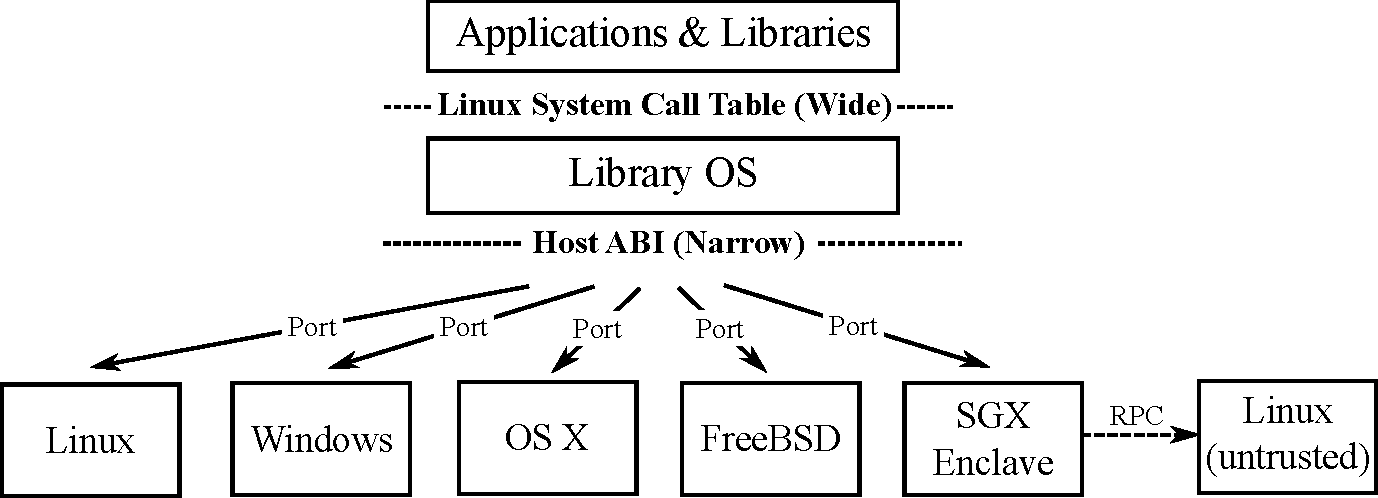
\includegraphics[width=30em]{porting.pdf}
\caption{Porting model of \graphene{}.}
%\vspace{-.1in}
\label{fig:overview:porting}
\end{figure}



\papersubsection{Platform Adaption Layers (PALs)}
\label{sec:overview:host:pal}


For each host OS or hardware, \graphene{} uses
a thin library called a {\bf platform translation layer (PAL)}
to translate among host interfaces.
%is loaded below the library OS, to translate each functions in \thehostabi{} to native system interfaces.
The main purpose of a PAL is to mitigate the semantic gap
between \thehostabi{} and
native host system APIs.
%The effort of PAL development is per host OS, whereas the library OS implementation is reusable on every hosts. %The simplicity of \thehostabi{} can be also estimated by the effort of implementing a PAL for each host.
By implementing a PAL on a new host OS or hardware,
users can reuse
the same \libos{} to run the same collection of unmodified Linux applications.
%To keep the porting effort low,
%the development of a PAL must be straightforward
%for average OS developers.
%to achieve with limited efforts.
%Based on the principle of porting simplicity, PAL development must be straightforward
%for average developers.







%The host ABI is defined for the simplicity of porting, as well as the sufficiency for implementing a library OS compatible to Linux.
%First of all, the number of host functions included in \thehostabi{}
%is much smaller than the number of system calls in a commodity OS such as Linux. 
\graphene{} currently contains PAL implementations for several popular OSes,
including Linux, \win{}, \osx{}, and FreeBSD.
%and \sgx{} with an untrusted Linux kernel.
Most of these OSes provide a POSIX-like system API similar to \thehostabi{}.
Due to the similarity, translating most of \thehostabi{} to one of the system APIs
are straightforward for average OS developers.
\Thehostabi{} is also much smaller than the actual POSIX API, making it extremely portable.



A part of \thehostabi{} may be challenging to port
on an OS,
due to unexpected system assumptions made by the OS.
For instance, \win{} does not support
fine-grained memory deallocation for de-privileged applications.
To implement system calls like \syscall{munmap} and \syscall{mprotect},
\graphene{} needs host ABIs to
deallocate or protect virtual memory pages at page granularity.
%A workaround is to change memory mappings at the physical page level,
%but will require running the \win{} PAL with root permissions.
%This type of porting challenges
%tends to be results of design decisions or assumptions made by OS developers.
%A \libos{} can potentially design
%different emulation strategies
%to compensate missing host abstractions.
A few host abstractions such as a bulk IPC feature are
optional to the host ABI;
if a host OS does not support these abstractions,
the \libos{} must fall back to alternatives. 

%In our experience, the development of a PAL is around ten thousand lines of code.

%For each port, the amount of code written for implementing \thehostabi{} is at the order of magnitude of thousands of lines of code, which is much more manageable than implementing a flat translation layer for system interfaces.


\begin{comment}
Based on the experience in \graphene{},
it is hard to ensure the portability of \thehostabi{} on every potential hosts.
%even a host ABI specialized for simplicity cannot guarantee to be portable on every hosts.
A host may simply lacks the functionality
for implementing a \hostapi{}.
The assumption is, maintaining the compatibility of \thehostabi{} poses a much less challenge than maintaining the whole system API.
Besides, the library OS may flexibly switch among emulation strategies
to compensate the absence of certain host abstraction.
As an example,
bulk IPC is optional in \thehostabi{} since its first definition,
due to the expectation
that implementing the feature may not be feasible on some hosts.
If bulk IPC is not available,
the library OS can fall back to RPC-based IPC, with a reasonable amount of performance penalty.
In the worst case, if there is no emulation strategies
to compensate for the absence of a \hostapi{},
user can predict the affected applications and avoid running these applications
on specific hosts. 
%at least users can predict whether an application will be affected and thus cannot run on certain hosts.
\end{comment}


%For a host OS that does not support ELF binaries, the PAL must follow the binary format which the host OS accepts, such as the Portable Executable (PE) format on \win{}.
%The PAL is the only layer in the user space which cannot be reused
%across different hosts. Besides the PAL, all of the other binaries in the user space are fully reusable, including the library OS, the supporting libraries, and the application executable.



%The host abstractions map to several common system calls in a commodity OS.
%For example, \funcname{StreamRead} and \funcname{StreamWrite} can directly map to the POSIX functions \funcname{pread} and \funcname{pwrite}, which are available in most OSes including Linux, BSD, \osx{}, and \win{}.
%More than half of the functions in \thehostabi{} can be counted toward this category.
%The rest of the host abstractions are either specific to Linux
%(e.g., TLS support),
%or belong to the POSIX functions that are not shared with commodity OSes
%(e.g., \funcname{mmap} on \win{}).
%The PAL emulates these host abstractions, using existing system interfaces available on the host OS, unless the software emulation is fundamentally impossible (e.g., restricted by the system interfaces), or too expensive (e.g., high overhead from copying data).



\papersubsection{Definitions and design principles}
 

\graphene{} defines \palcallnum{} calls in \thehostabi{} (also called \hostapis{}),
with a set of host abstractions
sufficient for \libos{} development.
%The host ABI defines the interaction between the library OS and a specific host.
%The \graphene{} library OS can be deployed on any ``host'' where \thehostabi{} has been ported.
This thesis defines
a {\bf host} of \thehostabi{}
to be an OS or hypervisor
which contains enough OS functionality for running a standalone application or virtual machine.
Most of the host targets in \graphene{}
are monolithic OSes,
including Linux, \win{}, \osx{}, and FreeBSD.
%which has defined a massive system API for programmability.
A monolithic OS 
usually contains a massive amount of system APIs,
which is sufficient for
implementing \thehostabi{}.


A special example of a host
is an \sgx{} (Software Guard Extensions) enclaves~\cite{intelsgx},
which
restricts OS functionality for security reasons.
The restrictions on \sgx{}
are results of a strong threat model
which distrusts any OS features except ones that are virtualized by the CPUs or migrated into enclaves.
The only way to obtain any missing OS features such as storage or networking
is to request through RPC (remote procedure call).
Requesting untrusted OS services through RPC also introduces new security threats that application developers tend not to anticipate~\cite{checkoway13iago,osdi16scone}.
Due to all the compatibility and security challenges discussed above,
this thesis uses \sgx{} as a representative example of a host
with unusual assumptions (e.g., threat models) and restrictions
compared to a monolithic OS.

%An innovative hardware abstraction like \sgx{} (software guard extensions)
%imposes unique assumptions and restrictions
%on a commodity OS,
%%creates a special host on top of Linux or \win{},
%%with unique interfaces and specifications regarding the host OSes.
%and thus creates a special host above the OS.

%If an OS has mutated or tweaked the interface for a hardware platform,
%such as an \sgx{} enclave 
%running on an untrusted Linux kernel,
%the combination of the OS (Linux) and the hardware platform (\sgx{}) is considered a specialized host.
%Especially, the \sgx{} port of \thehostabi{} faces several unique challenges,
%which will be discussed in Chapter~\ref{chap:sgx}.


\begin{comment}
%\fixme{each sentense should be a paragraph; starting the 2nd sentence}
\fixmedp{start with a strong opening stating the rationale}
The host ABI of \graphene{}
define functions needed from a host, in order to implement the library OS for reusing applications.
%to reuse an application and all its supporting libraries, including the \graphene{} library OS.
Each host of \graphene{} contains an OS and a hardware platform, either of which causes compatibility issues for running unmodified applications.
OS developers can port the library OS to a new host,
by simply reimplementing the narrowed host ABIs using abstractions available on the host.
%a new host platform.
%For each host which requires the compatibility for unmodified Linux applications, one only has to implement the narrowed host ABIs,
%instead of reimplementing the bloated, ``legacy'' system interfaces
%needed by the applications.
By implementing \thehostabi{}, OS developers skip the painful process of rebuilding the whole system interfaces of a commercial OS such as Linux.
The host ABIs strictly decouples the porting effort on the hosts from the compatibility feature for applications.
%The host ABIs decouple the OS development in the host and the implementation of compatibility for the existing Linux application.
What \thehostabi{} exposes is a simplified extended machine,
similar to a para-virtualization interface, capable of running the library OS as a lightweight virtual machine. % with compatibility against Linux applications.
%on which another layer of virtualization (i.e., the library OS) can be built to reproduce the compatibility for Linux.
\end{comment}


\begin{comment}
Two design principles drive the definition of \thehostabi{}s:
{\em simplicity} (i.e., easy to port on any hosts)
and {\em sufficiency} (i.e., containing enough OS functions for implementing a library OS).
The process of deciding \thehostabi{}s is comparable to
finding a ``pinch point'' within a OS implementation,
which can conveniently mediate a significant portion of OS execution paths for managing hardware abstractions.
%The two principles drive the development of \thehostabi{}s,
%The whole development of the \graphene{} library
%must be disciplined
%on extending \thehostabi{}s only when it is strongly required.
%of restraining extensions to \thehostabi{}s unless absolutely necessary.
The two principles
determine the soundness of the \graphene{} approach to improving compatibility
for any hosts.
\end{comment}


%%The host ABI is defined with partitioning in mind.
%\Thehostabi{} 
%determines a boundary which partitions several upper-level OS components, %, such as system calls and namespaces,
%into a library OS,
%%, as a dynamically-linked library which can be deployed
%%to various hosts.
%%The rationale behind the partitioning is based on the fact that not every OS component is equally important to compatibility, for applications which need to be ported across hosts.
%%When an OS is extended for a new hardware,
%%these OS components usually remain unchanged, or are predominantly reused.
%%Partitioning
%%into a library OS further guards these 
%in order to isolate the host idiosyncrasy. % on specific hardware. %any potential changes for adopting new hardware.
%%Similar isolation
%%exists in traditional OSes, but without partitioning:
%The strategy
%is also used in OSes:
%An example is the Linux virtual file system (VFS), an internal interface
%which encapsulates operations of file system drivers.
%%On the other hand,
%%drivers (e.g., drivers for file systems, block devices, or network cards)
%%and architecture-specific instructions
%%stay encapsulated in the host OS.
%%in the Linux kernels are usually encapsulated under a virtualized, in-kernel interface (e.g., the Linux virtual file system),
%%to simplify the development of the rest of the kernel.
%Similar to VFS,
%\thehostabi{} is intended
%to be a more ubiquitous interface,
%which encapsulates
%any host-specific behavior and semantic
%inside the host OS.
%%for encapsulating both OS and hardware idiosyncrasy on a wide range on hosts.
%%declares a ubiquitous system interface, to encapsulate both OS and hardware abstractions
%%for the library OS.




\Thehostabi{} shares several characteristics with a virtual hardware interface
exported by a hypervisor.
A generic, backward-compatible
virtual hardware interface
%a set of generic, virtual hardware,
%which the VM can control with the same drivers.
allows an unmodified OS kernel to run inside a virtual machine as on the bare metal.
%by exporting interfaces close to commodity hardware.
%To avoid additional porting effort, the virtual hardware are close to the typical commodity hardware.
%For instance, a virtual hardware interface
%usually includes a virtual NIC (network interface controller),
%such as the virtualized E1000 interfaces
%available in VMware workstation or QEMU.
%As a result, \thehostabi{} contains the
%typical OS features and interfaces, similar to the API of early UNIX systems.
The key difference between
a virtual hardware interface
and \thehostabi{}
is that \thehostabi{} does not target reusing a whole, unmodified OS kernel as a guest.
Instead, 
\thehostabi{} contains higher-level abstractions such as files and network sockets
to ensure portability on most host OSes.
The concept
of defining \thehostabi{}
with a customized guest OS (i.e., a \libos{}) running atop \thehostabi{} is similar to para-virtualization.
%\thehostabi{} expects the \libos{}
%to be rewritten and
%customized for \thehostabi{},
%similar to a 
%para-virtualizated VM.
%Compared to an actual para-virtualized VM,
A para-virtualized VM defines hypercalls as interfaces between a guest OS and a hypervisor.
Furthermore, \thehostabi{} avoids duplication of OS components
such as scheduler, page fault handler, file systems, and network stacks
between the host and \libos{}.
%Another difference is that \thehostabi{} is called by normal function calls, whereas para-virtualization relies on hypercalls.
To compare a VM and a \libos{} on a spectrum,
a VM reuses a whole OS on a wide, backward-compatible virtual hardware interface
whereas a \libos{} implements only system API components on a simplified host ABI.

The following paragraphs discuss the key design principles of \thehostabi{},
including porting simplicity, sufficiency for \libos{} development, and ease of migration.

\paragraph{Porting simplicity.}
%To reduce porting effort
%\thehostabi{}
%must be simple to port on a host OS or hardware.
To reduce porting efforts,
\graphene{} defines \thehostabi{}
using two strategies:
first, \graphene{} significantly reduces both the size and complexity of host OS features
that OS developers have to implement.
Effectively, \graphene{} avoids duplicated OS features and handling rare corner cases
on \thehostabi{}.
%The development of \graphene{} disciplinarily avoiding adding any functions to \thehostabi{},
%unless the library OS cannot internally implement an OS feature.
Second, the definition of \thehostabi{}
imitates common system APIs in a POSIX-like monolithic OS,
to directly translate most calls to
a few similar host abstractions.
%existing system calls or system library functions
%on each host.
%include functions which can be directly mapped to OS functions exported by the host.
%%the likelihood of finding similar features on the host, to be translated to functions in \thehostabi{}.
%The assumption that such a strategy is possible
%is based on
%the observation that
%%similarity of system interfaces is common among most OSes.
%similar OS functions, especially UNIX-style APIs,
%tend to commonly exist in most OSes.
%, to reduce the learning curve for programming applications.
For instance,
the stream APIs in \thehostabi{}, such as \palcall{StreamRead} and \palcall{StreamWrite}
are similar to
system calls like \syscall{read} and \syscall{write} exist on Linux, BSD, and POSIX API,
or \syscall{ReadFile} and \syscall{WriteFile}
on \win{}.
%with similar functionality and semantics.
%and 
%looks similar to \syscall{ReadFile} in \win{}, except the data types.
%The definition of \thehostabi{}
%is based on observations of the system interfaces in some of the important hosts,
%including Linux system calls and \win{} API.
%exported by the targeted hosts,
%and defines the functions in \thehostabi{}, to be easily translated to the native system interfaces.
%The host ABI is essentially a subset of the common features from every potential hosts.
%We expect %\thehostabi{} defined with simplicity in mind
%to be straightforward to port on most hosts,
%Most functions in \thehostabi{} can be easily translated to host system interfaces
%in various styles.
As the rest of this thesis proves, porting \thehostabi{} is straightforward
on most monolithic OSes.

%For example, \thehostabi{} defines \syscall{StreamRead} and \syscall{StreamWrite} for accessing I/O streams, similar to .
%xcept some nuanced details like order of parameters.


% by including OS functions , such as \syscall{FileRead} and \syscall{FileWrite}, similar to the Linux system calls, \syscall{pread} and \syscall{pwrite}.




\begin{comment}
The simplicity of \thehostabi{}s requires retaining a minimalist design of host functions. %, based on typical OS services for managing hardware.
%\graphene{} reduces the host functions
%to the bare minimum.
The host ABIs should only contain operations that
are absolutely necessary for requesting external hardware abstractions.
%A way to simplify \thehostabi{}s is to move host functions into the library OS
%and to replace them with wrappers consisting of other host functions.
Any functions that can be partially or wholly implemented inside the library OS
should be further simplified, or even removed from \thehostabi{}s.
%---in other words, whether \thehostabi{}s can be further reduced.
Moreover, \thehostabi{}s have to be simple enough to implement on
most hosts;
%In the simplest host ABIs, none of the host functions shall be able to internally implement the behavior of another host function,
%or the definition of \thehostabi{}s is further reducible.
that is, \thehostabi{}s should contain only OS functions that are commonly offered on
most hosts.
The host ABIs are close to simplified UNIX interfaces,
such as reading or writing a file or an I/O device as a byte stream,
or creating a virtual memory mapping.
%the most common OS functions
%offered on most of the potential hosts,
For most hosts,
implementing \thehostabi{} should be as straightforward as redirecting the functions to the closest host system calls.
%such as the Linux system calls or the \win{} APIs.
For example, the functionality of \syscall{StreamRead} and \syscall{StreamWrite} in \thehostabi{}s can loosely match with
\syscall{read} and \syscall{write} in Linux,
or \syscall{ReadFile} and \syscall{WriteFile} in \win{}.
%This thesis also evaluates the simplicity of \thehostabi{}s by counting the lines of code used to implement \thehostabi{}s on each host platforms.
Since most OSes have inherited a similar design from UNIX,
it is fair to assume finding
comparable OS functions %host platforms
to \thehostabi{} would be reasonably easy.
%fair to assume that \thehostabi{}s 
\end{comment}



\paragraph{Sufficiency for \libos{} development.}
%\Thehostabi{} defines
%the host abstraction available for a \libos{} to access host hardware abstractions.
To develop a \libos{} with compatibility against a wide range of applications,
\thehostabi{}
%are demonstrated by the fact that
%the exported host functions 
contain any OS abstractions that the \libos{} cannot easily emulate.
%and a full-function library OS is implemented on top of them.
For most hosts,
the host OS abstractions
%can be categorized into five types:
include
process creation, memory management, and I/O (typically, files and network connection)~\cite{dhamdhere2007os-textbook}.
%Besides security and protection,
%the definition of \thehostabi{} is closely related with hardware management,
%and offers the most basic abstractions for each category of OS functions.
%managing specific types of hardware,
%and each contain a few basic abstractions
%which can be expanded into other system interfaces.
%For example, the basic OS functions for memory management include
%allocating (\syscall{VirtMemAlloc}),
%protecting (\syscall{VirtMemProt}),
%and deallocating (\syscall{VirtMemFree}) memory regions. % at certain granularity
%(usually in pages).
%These basic functions can be used to implement other forms of memory allocation,
%such as growing heaps with \syscall{brk}
%or allocating thread-private stacks.
%The definition of the \drawbridge{} host ABI is a hint, for creating a list of host abstractions necessary for the library OS, including streams, memory, threads, and processes. 
%If \thehostabi{}s are insufficient for implementing certain system interfaces, one may extend \thehostabi{}s with the missing functions,
%with the discipline to retain the simplicity of \thehostabi{}s.
%The extension to \thehostabi{}s must be d, to keep the extension minimal, and to avoid adding redundant functions.
%The implementation of the \graphene{} library OS demonstrates that
%\thehostabi{} is sufficient for implementing significant portion of Linux system calls.
For each type of abstractions,
a monolithic OS may define several variants of system APIs with similar functionality.
For instance, Linux provides two system calls, \syscall{mmap} and \syscall{brk}, both for memory allocation in a process.
\syscall{mmap} allocates larger memory regions with page granularity,
whereas \syscall{brk} simply grows a single, continuous heap space for more fine-grained allocation.
Many applications such as GCC~\cite{gcc}
switch among system API variants in case one of them is unavailable on certain OS distributions.
This thesis shows that,
by adopting only the semantics of one of these similar APIs or abstractions, the host OS can stay simple with
the \libos{} emulating the rest of APIs.
For instance, \thehostabi{} includes \syscall{VirtMemAlloc}
as a similar feature as \syscall{mmap},
which is sufficient to emulating both \syscall{mmap} and \syscall{brk}.



\graphene{} defines \thehostabi{} partially based on
\drawbridge{},
a library OS for single-process \win{} applications.
The host ABI of \drawbridge{} 
contains 36 functions,
%demonstrates that its host ABI is sufficient
%for running a library OS in which 99.7\% of code comes from the \win{} 7 source.
%The host ABIs of \drawbridge{} are later extended
%for running a Linux-based library OS called Bascule~\cite{baumann13bascule}.
and several works have ported the host ABI to different hosts,
including \win{}, Linux, Barrelfish, and \sgx{}~\cite{porter11drawbridge,baumann14haven,mssql-on-linux,baumann13bascule}.
%and is capable of running a library OS for single-process, Linux applications, with a few host ABI changes~\cite{baumann13bascule}.
%ill loads and links the rest of application binaries, just like the native Linux loader (i.e., \code{ld.so}).
%\graphene{} takes the high-level definitions of the \drawbridge{} and Bascule host ABIs, and customizes for general-purpose Linux applications and a wider range of hosts. 
Although running \win{} and Linux applications may face
a different set of challenges,
the nature of their APIs is mostly similar, with a few exceptions.
During the development of \graphene{}, developers found the occasions in which
the host ABI of \drawbridge{}
is not sufficient to address Linux-specific challenges
and decide to extend \thehostabi{}.
Section~\ref{sec:overview:host:abi} and Chapter~\ref{chap:abi}
will further discuss the Linux-specific extensions of \thehostabi{}.


\paragraph{Migration.}
The \graphene{} library OS shares several features of VMs, including checkpointing and migrating a running application.
Migrating a process is also the key to emulating copy-on-write forking,
on a host without physical memory sharing (e.g., \sgx{}).
A hypervisor checkpoints and migrates a VM by snapshotting the VM states above a stateless virtual hardware interface. % as a clean boundary for snapshotting the application and OS state.
\Thehostabi{} is also defined to be statelessness,
by ensuring any states in the hosts to be temporary and reproducible to the applications and \libos{}.





\papersubsection{The \hostapis{}}
\label{sec:overview:host:abi}


%\fixmedp{the beginning doesn't capture the whole paragraph.}
%The host ABI shares several common abstractions with production OSes.
%The functions in \thehostabi{}
%define the basic features needed from the hosts, to run the library OS.
%The definition of the host functions
%should be unsurprising to average OS developers,
%making the implementation on a new host to be fairly straightforward.
%The host ABI reflects the common functionality of most OSes, including Linux and \win{}.
%Although the same OS abstractions may be defined
%as different idiosyncratic system interfaces on each host OSes,
%\graphene{} takes into consideration of porting the host functions to either OSes, in the most effortless way possible.





%fixmedp{give more of the background}
Table~\ref{tab:overview:abi} lists the \palcallnum{} calls defined in \thehostabi{}:
%Among these \hostapis{}, 
25 calls are inherited from the \drawbridge{} host ABI,
including functions to managing I/O (e.g., \palcall{StreamOpen}), memory allocation (e.g., \palcall{VirtMemAlloc}), scheduling (e.g., \palcall{ThreadCreate}), and several miscellaneous functions (e.g., \palcall{SystemTimeQuery}).
%Most of the host functions only affect the OS or hardware states
%related to the process itself.
%For example, \syscall{VirtMemAlloc} can only allocate memory in the calling process,
%and cannot affect other processes running in parallel.
%Only I/O streaming functions export states to the host OS, and share states with other processes or library OSes.
14 calls are added by \graphene{}, to implement Linux-specific features.
For example, unlike \win{} or \osx{}, Linux %The host ABI is also complemented with several Linux-specific abstractions, such as
delivers hardware exceptions to a process as signals.
Linux also requires 
the x86-specific segment registers (i.e., FS/GS registers)
to determine the location of thread-local storage (TLS), which can be hard-coded in application binaries by a compilation mode of GCC.
On \win{} or \osx{}, the x86-specific segment registers are mostly ignored, and even frequently reset to eliminate attack vectors.
%The host ABI contains host functions (), which can be directly called from the library OS. \graphene{} shows that \thehostabi{} is sufficient to implementing a large portion of the Linux system calls.
%These functions are not defined in \drawbridge{}, the \win{}-based library OS,
%because these abstractions do not exist in \win{}.
%The \drawbridge{} host ABI does not contain exception delivery because the feature is
%not commonly used in \win{} applications.
%Moreover, the x86 segment registers cannot be modified in \win{}
%because the OS assigns fixed values to these registers
%for the whole execution.
%Although \drawbridge{} excludes these abstractions, Bascule extends \thehostabi{} to include similar functions,
%demonstrating that the extension is indeed necessary.
\graphene{} discovers these abstractions as a necessity for implementing a rich Linux \libos{}.



\begin{table}[htp!]
\centering
\small
\begin{tabular}{|p{.15\textwidth}|p{.33\textwidth}|p{.45\textwidth}|}
\hline
{\bf Abstraction} & {\bf Function Names} & {\bf Description} \\
\hline
\raggedright
Streams & 
\raggedright
{\tt StreamOpen} \newline
{\tt StreamMap} \newline
{\tt StreamFlush} \newline
{\tt StreamSetLen} \newline
{\tt StreamRead} \newline
{\tt StreamWrite} \newline
{\tt StreamWaitforClient} \newline
{\tt StreamAttrQuery} \newline
{\tt StreamAttrQuerybyHandle} \newline
{\tt StreamAttrSetbyHandle} \newline
{\tt StreamDelete}
& 
Opening streams using URIs, with prefixes representing stream types (e.g., \code{file:},\code{tcp:},\code{pipe:}),
as well as common stream operations, including transmission of data, and query to the stream attributes.
\\
\hline
\raggedright
Memory & 
\raggedright
{\tt VirtMemAlloc} \newline
{\tt VirtMemFree} \newline
{\tt VirtMemProtect}
& 
Allocation, deallocation, and protection of a chunk of virtual memory.
\\
\hline
\raggedright
Threads \& scheduling & 
\raggedright
{\tt ThreadCreate} \newline
{\tt ThreadExit} \newline
{\tt ThreadDelayExecution} \newline
{\tt ThreadYieldExecution} \newline
{\tt SemaphoreCreate} \newline
{\tt SemaphoreRelease} \newline
{\tt EventCreate} \newline
{\tt EventSet} \newline
{\tt HandlesWaitAny}
&
Creation and termination of threads; 
Using scheduling primitives, including suspension, semaphores, events, and pollable IO events.
\\
\hline
\raggedright
Process & 
\raggedright
{\tt ProcessCreate} \newline
{\tt ProcessExit}
& 
Creating or terminate a process with a library OS instance.
\\
\hline
\raggedright
Mis\-cel\-la\-ne\-ous & 
\raggedright
{\tt SystemTimeQuery} \newline
{\tt RandomBitsRead}
& 
Querying system time, and random number generation.
\\
\hline
\raggedright
Exceptions $\dagger$ & 
\raggedright
{\tt SetExceptionHandle} \newline
{\tt ExceptionReturn}
& 
Setting an exception handler, and returning from the handler.
\\
\hline
\raggedright
TLS $\dagger$ & 
\raggedright
{\tt SetSegmentReg}
& 
Setting the \code{FS}/\code{GS} registers.
\\
\hline
\raggedright
Remote Procedure Call $\dagger$ (optional)& 
\raggedright
{\tt StreamSendHandle} \newline
{\tt StreamRecvHandle} \newline
{\tt CreateIpcChannel} \newline
{\tt PhysicalMemoryCommit} \newline
{\tt PhysicalMemoryMap}
& 
Sending opened stream handles or physical memory across processes.
\\
\hline
\end{tabular}
\caption{An overview of \thehostabi{} of \graphene{}. The ones marked with the symbol $\dagger$ are introduced in the initial publication of \graphene{}~\cite{tsai14graphene} or later extended for this thesis. The rest are inherited from \drawbridge{}~\cite{porter11drawbridge}.}
\label{tab:overview:abi}
\end{table}

%The interfaces, as part of \thehostabi{}, which access these host abstractions, are ultimately simplified to reduce the porting effort on each host.
%Unlike the system interfaces in the OS, \thehostabi{} does not prioritize backward compatibility. Therefore, \thehostabi{} includes only the minimum interfaces that the library OS needs to interact with the host. The host ABI does not have to include any of  the legacy system interfaces from a production OS, let alone preserving different flavors of system interfaces for backward compatibility.



\graphene{} introduces five calls for 
remote procedure call (RPC) between \libos{} instances
in a multi-process application.
\graphene{} simplifies porting multi-process abstractions
on each host OS
to implementing RPCs.
The basic RPC abstraction is 
a pipe-like RPC stream for message passing between processes.
To improve performance,
%RPC is critical for implementing the coordination of OS states
%across library OS instances.
%The basic form of RPC in \graphene{} is a pipe-like RPC byte stream, which a library OS can simply use to send messages.
%It is a common design choice
%to implement inter-process coordination through message-passing
%instead of shared memory, especially for hardware platforms that do not guarantee memory coherence~\cite{baumann09barrelfish}.
%A problem to the message-passing approach is the significant overheads
%on frequently exchanging distributed OS states.
\thehostabi{} defines an optional, bulk IPC abstraction
to send large chunks of virtual memory
across processes.
%The bulk IPC feature works similarly as sending the memory through RPC streams,
%but is much faster because it avoids copying memory in the host.


%for host platforms that urgently require lowering the RPC overheads.
%Another extension is for
%%\funcname{StreamSendHandle} and \funcname{StreamRecvHandle}
%delegating opened stream handles to another process, through a connecting pipe.
%The feature is similar to sending file descriptors
%through UNIX sockets in Linux, and is used to share opened network sockets with the \syscall{fork}'ed processes.
%%Another RPC abstraction is a bulk IPC channel; a process can use \funcname{PhsyicalMemoryCommit} to commit a large chunk of memory to a bulk IPC channel, which \funcname{PhsyicalMemoryMap} can map into another process, as copy-on-write. The library OS uses bulk IPC as an optimization to \syscall{fork}.
%Despite that either of the RPC primitives
%is not necessary easy to implement on every hosts, the inclusion of these host functions is completely optional, and the library OS can always fall back to the message-passing approach.



%All the host functions are designed to appear as ``stateless''
%as possible to the library OS.
%Being stateless to the library OS means that
%a host function does not preserve any permanent state of certain host abstraction.
%A stateless function can recover
%from disconnection of the library OS, and be reconnected at any timing.
%The host functions can maintain temporary bookkeeping for the convenience of porting,
%but should not assume the bookkeeping states to be permanent.
%The principle of defining all the host functions to be stateless
%is primarily for two purposes:
%{\em migration} and {\em security isolation}.
%For migration, the fact that the library OS can disconnect freely from the host functions simplifies the implementation of the migration feature.
%Migration is also an important foundation to implementing \syscall{fork}, because the cloned process need to receive a snapshot of the parent process.
%For security isolation, 
%a stateless host function is easier to check,
%because the security monitor only has to verify each instance of host function calls,
%instead of tracing multiple host functions over a longer period of time.

%the functions to access each host abstraction must appear \fixmedp{clarify `stateless'} stateless to the host, except for the handles to identify the resources. Each call to the host functions is independent. The arguments given for each call must be always be absolute values, instead of relative values.
%For example, the offset given to \funcname{StreamMap}, \funcname{StreamRead}, and \funcname{StreamWrite} (if the opened handle is a file) are offsets from the beginning of the file, and thus are irrelevant to how many bytes that are previously written or read.
%When enforcing isolation rules, the host OS can check the arguments of each calls to the host functions, independently and atomically.


%A host ABI (application binary interface) has to define the convention of application binaries, including the binary format and the linking procedure, as well as a set of  system interfaces.
%The host ABIs contain a minimal loader which recognizes a basic version of the ELF (Executable and Linkable Format), just enough to compose a binary of the library OS.
%The very initial loading procedure as part of \thehostabi{}s only loads a clean library OS instance.
%Each host of \graphene{} is supposed implement a minimal dynamic loader,
%which can load the \graphene{} library OS binary in ELF.
%The library OS then completes the dynamic loading procedure,
%by directly loading the Linux native dynamic loader (i.e., \code{ld.so}), and indirectly loading the rest of the application binaries.







\papersubsection{Host-enforced security isolation}
\label{sec:overview:host:security}


To target multi-tenant environments, 
\graphene{} enforces strong security isolation between mutually-untrusting applications running on the same host.
The security isolation of \graphene{} is comparable to running each application
in a VM or a container.
Just as a virtual hardware interface isolating each VM,
\thehostabi{} also enforces security isolation between library OS instances.
%according to the trust model of the applications.


On a trusted host OS,
\graphene{} delegates security isolation as a host-level feature.
The library OS and the application must mutually trust each other, due to lack of internal privilege separation in a process.
%The host ABI also separates API implementation
%from security isolation.
%To ensure isolation, each host must restrict access from the applications or the library OS, to any unauthorized host abstractions.
On each host, a reference monitor enforces security isolation policies, by access control on OS abstractions sharable among processes, including files, network sockets, and RPC streams.
%The host-level security isolation is orthogonal to API complexity.
Separating security isolation from API implementation simplifies security checks
for applications that only require
complete protection from other tenants.
%based on monitoring the references to host resources and rejecting authorized resource access.
%to the host abstractions.





%\graphene{} reduces the attack surface exposed to applications
%by restricting access to the host kernel ABI 
%and prevents access to unauthorized system calls, files, byte streams,
%and network addresses with a \emph{reference monitor}.
%The host kernel ABI exported by the \pal{} heavily 
%limits the ability of a \graphene{} application to interact with the rest of the system;
%any external interactions are further mediated by a reference monitor.
%Unlike a typical Linux system, \graphene{} applications cannot interact with shared 
%system daemons or other shared system resources.
%As a result, \graphene{} enforces security isolation similar to running applications in separate VMs---even
%applications that span multiple processes.


In \graphene{},
one or multiple processes of the same application run in a {\bf sandbox}.
Multiple library OS instances coordinate
in a sandbox
to present a unified OS view
to the application.
%As the library OS instances can coordinate shared OS states using simple RPC streams,
The design simplifies the enforcement of security isolation for multi-process abstractions.
\graphene{}
uses the reference monitor to block RPC streams across the sandbox boundary,
stopping applications in different sandboxes from accessing multi-process OS states.
%\graphene{} contributes a multi-process security model 
%based on the abstraction of a \emph{sandbox},
%or a set of mutually trusting processes.
%If a reference monitor exists, the reference monitor permits the processes within the same sandbox to communicate and exchange RPC messages, but disallows cross-sandbox communication.
The current design focuses on security isolation, although we do expect to extend the design for more sophisticated policies
in the future.

\begin{comment}
The only host abstractions that are shared across processes and must be mediated by the host for isolation are files, network sockets, and RPC streams
--- all other allowed host ABI modify only local process state, such as VMAs and threads.
%Thus, the reference monitor need only mediate file access, socket and RPC stream creation.
%an unprivileged daemon
%as well as extensions to the App\-Armor LSM~\cite{apparmor},
%which checks file and socket policies in the kernel.
%, reducing context switching overhead
%and the risk of race conditions~\cite{garfinkel03traps}.
In order for the reference monitor to restrict file access, socket and RPC stream creation,
each application includes a {\em manifest file}~\cite{hunt07rethink},
which describes a {\tt chroot}-like, restricted view of the local 
file system (similar to Plan 9's unioned file system views~\cite{pike90plan9}),
%including read-only shared files,
as well as {\em iptables}-style~\cite{iptablesman} network firewall rules.
To facilitate sharing read-only libraries, a manifest may specify a file system view which combines several different sub-directories of the local file system, and can prevent writing to files or directories.


For example, the \graphene{} reference monitor on the Linux host is implemented using \syscall{ioctl} to a special device (\code{/dev/graphene})~\fixme{a prospective design}.
A process is restricted by the Linux BPF-style system call filter, or the SECCOMP filter~\cite{seccomp}, to use \syscall{open} to access any files, or to \syscall{connect} or \syscall{bind} to any sockets.
It must use the \graphene{} special device to open or create streams, so the file paths or network addresses can be checked against the sandbox rules. The kernel module as the driver of the \graphene{} special device can coexist with any Linux Security Module (LSM), such as AppArmor~\cite{apparmor} or SELinux~\cite{selinux}.


When a new process is launched by the host, it begins execution in a new sandbox.  
Child processes may either inherit their parent's sandbox, or can be started in a separate sandbox---specified by a flag to the host abstractions of process creation.
A parent may specify a subset of its own file system view 
when creating a child, but may not request access to new regions of the host file system. 
%The restrictive policy enforced on the child will be written in a new manifest file generated by the parent, and the policy will be checked by the reference monitor.
The child may also issue an {\tt ioctl} call to 
dynamically detach from the parent's sandbox. The reference monitor prevents byte stream creation across sandboxes.
%among picoprocesses
%that are not in the same sandbox.
%and restricts external connections to remote URIs according to firewall rules in the manifest.
When a process detaches from a sandbox, effectively splitting the sandbox, the host must closes all RPC streams that could bridge the two sandboxes.
\end{comment}



\paragraph{Threat model.}
For most hosts, application trusts the host OSes as well a \libos{} instances in the same processes.
For multiple processes inside a sandbox,
the \liboses{} in these processes
also trust each other.
Applications or \liboses{} are not trusted by the host OSes or processes outside of the sandboxes.
Applications and \liboses{}
can become the adversary to the host OS,
by exploiting vulnerabilities on \thehostabi{}.
%the \graphene{} design reduces the attack surface between the hosts and the library OS instances, to defend against a malicious application.

%On a host with a reference monitor, the host OS and the reference monitor are both trusted, to mediate all system interfaces used to implement \thehostabi{}. The host must check all access to any abstractions with effects outside of a process's internal state, such as an opened file, or a connected network socket.
%Processes inside the same sandbox mutually trust each other. The adversary can run arbitrary code inside of one or more processes within one or more sandboxes.
%The adversary can control all code in its processes, including the library OS and the host-specific PAL.
%{\tt libLinux} and the \pal{}. 
%We also assume a trusted reference monitor process running on the host kernel that 
%launches \graphene{} applications and mediates all system calls with external effects,\fixmedp{define precisely}

%\graphene{} ensures that %The key security property the \graphene{} design upholds is that 
%the adversary cannot interfere with any victim picoprocesses
%in a separate sandbox.  
%The \graphene{} sandbox design ensures strict isolation: 
%if the only shared kernel abstractions are byte streams and files, 
%and the reference monitor ensures
%there is no writable intersection between sandboxes,
%the adversary cannot interfere with any victim picoprocess.


The threat model of \graphene{} on \sgx{}
contains the adversary from other hosts but excludes
the host OS, hypervisor, and any hardware except the CPU from its trusted computing base (TCB).
An untrusted OS or hypervisor
potentially has lots of opportunities to invade applications or VMs,
using Iago attacks~\cite{checkoway13iago}.
The challenges of porting \graphene{} to \sgx{} is not limited to resolving the compatibility issues of enclaves but also defending applications and \liboses{} against untrusted host OSes.







%%% The only processes allowed to run as standard kernel processes (non-\graphene{}) 
%%% are the reference monitor and
%%% system administration utilities that need more kernel interfaces than the \pal{} ABI provides.
%%% Ensuring that a collaborating picoprocess correctly implements
%%% some function (such as receiving a signal),
%%% as well as preventing exploitation of vulnerabilities in picoprocesses
%%% are beyond the scope of this work.

%\graphene{} reduces the system attack surface of the host, but does not change the size of its
%trusted computing base; however, reducing the effective system call table
%size of a picoprocess does facilitate adoption of a smaller host kernel,
%which we leave for future work.




